\documentclass[tikz,border=12pt]{standalone}
\usepackage[utf8]{inputenc}
\usepackage{tikz}
\usetikzlibrary{shapes,arrows.meta,positioning,calc}

\definecolor{ScoutGreen}{HTML}{005432}
\definecolor{ScoutNavy}{HTML}{002855}
\definecolor{ScoutBlue}{HTML}{006EB6}
\definecolor{ScoutRed}{HTML}{A31920}
\definecolor{ScoutAmber}{HTML}{D97706}
\definecolor{BorderGray}{HTML}{CBD5E1}

\begin{document}
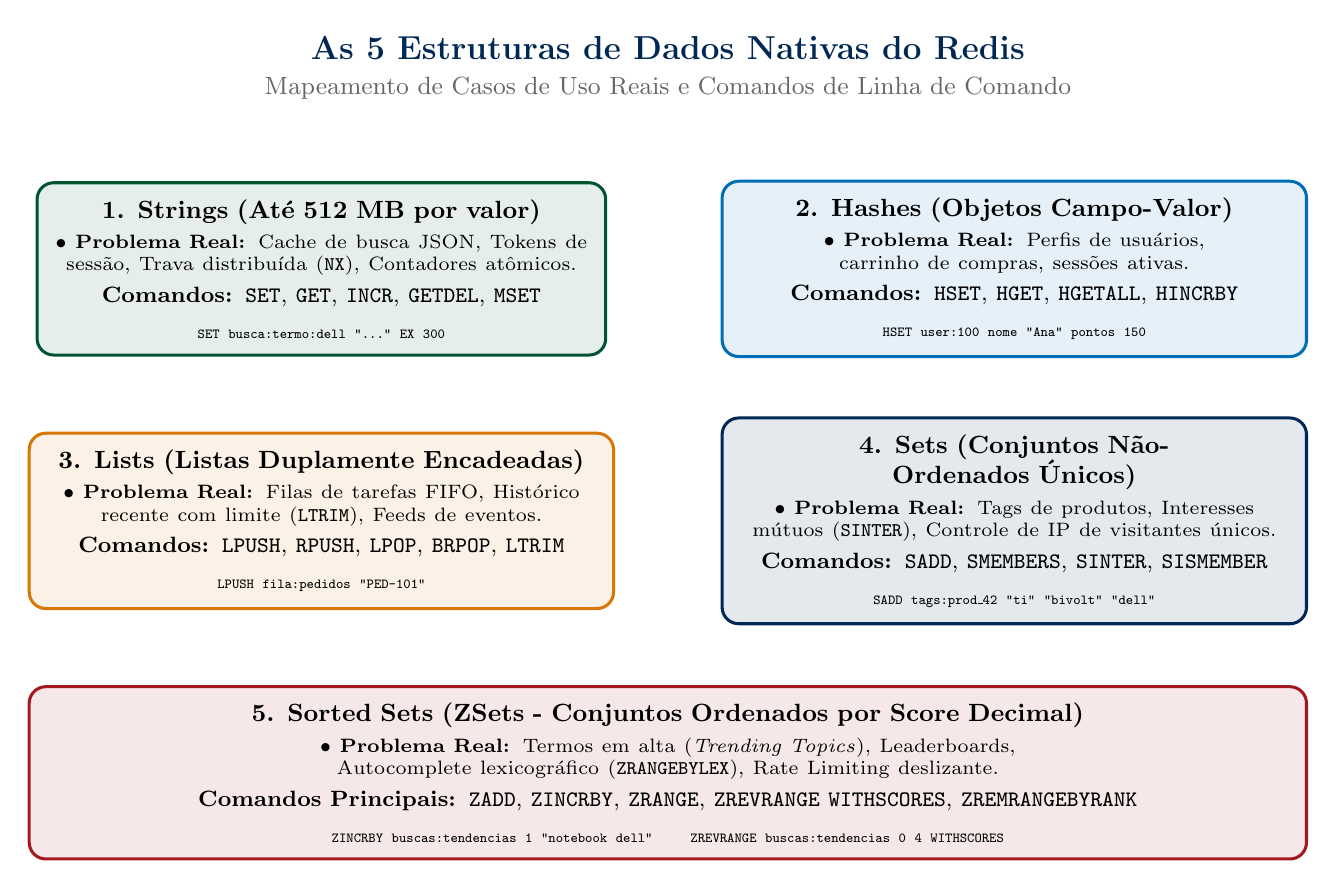
\begin{tikzpicture}[
    font=\sffamily,
    box/.style={draw=BorderGray, rounded corners=6pt, fill=white, line width=1.1pt, align=center, inner sep=6pt}
]

  % Título
  \node[font=\bfseries\large, text=ScoutNavy] at (8.0, 8.2) {As 5 Estruturas de Dados Nativas do Redis};
  \node[font=\small, text=gray!80!black] at (8.0, 7.7) {Mapeamento de Casos de Uso Reais e Comandos de Linha de Comando};

  % 1. STRINGS
  \node[box, fill=ScoutGreen!10, draw=ScoutGreen, text width=6.8cm, font=\small] (s1) at (3.6, 5.4) {
    \textbf{1. Strings (Até 512 MB por valor)}\\[3pt]
    \scriptsize $\bullet$ \textbf{Problema Real:} Cache de busca JSON, Tokens de sessão, Trava distribuída (\texttt{NX}), Contadores atômicos.\\[2pt]
    \footnotesize \textbf{Comandos:} \texttt{SET}, \texttt{GET}, \texttt{INCR}, \texttt{GETDEL}, \texttt{MSET}\\[2pt]
    \texttt{\tiny SET busca:termo:dell "{...}" EX 300}
  };

  % 2. HASHES
  \node[box, fill=ScoutBlue!10, draw=ScoutBlue, text width=7.0cm, font=\small] (s2) at (12.4, 5.4) {
    \textbf{2. Hashes (Objetos Campo-Valor)}\\[3pt]
    \scriptsize $\bullet$ \textbf{Problema Real:} Perfis de usuários, carrinho de compras, sessões ativas.\\[2pt]
    \footnotesize \textbf{Comandos:} \texttt{HSET}, \texttt{HGET}, \texttt{HGETALL}, \texttt{HINCRBY}\\[2pt]
    \texttt{\tiny HSET user:100 nome "Ana" pontos 150}
  };

  % 3. LISTS
  \node[box, fill=ScoutAmber!10, draw=ScoutAmber, text width=7.0cm, font=\small] (s3) at (3.6, 2.2) {
    \textbf{3. Lists (Listas Duplamente Encadeadas)}\\[3pt]
    \scriptsize $\bullet$ \textbf{Problema Real:} Filas de tarefas FIFO, Histórico recente com limite (\texttt{LTRIM}), Feeds de eventos.\\[2pt]
    \footnotesize \textbf{Comandos:} \texttt{LPUSH}, \texttt{RPUSH}, \texttt{LPOP}, \texttt{BRPOP}, \texttt{LTRIM}\\[2pt]
    \texttt{\tiny LPUSH fila:pedidos "PED-101"}
  };

  % 4. SETS
  \node[box, fill=ScoutNavy!10, draw=ScoutNavy, text width=7.0cm, font=\small] (s4) at (12.4, 2.2) {
    \textbf{4. Sets (Conjuntos Não-Ordenados Únicos)}\\[3pt]
    \scriptsize $\bullet$ \textbf{Problema Real:} Tags de produtos, Interesses mútuos (\texttt{SINTER}), Controle de IP de visitantes únicos.\\[2pt]
    \footnotesize \textbf{Comandos:} \texttt{SADD}, \texttt{SMEMBERS}, \texttt{SINTER}, \texttt{SISMEMBER}\\[2pt]
    \texttt{\tiny SADD tags:prod\_42 "ti" "bivolt" "dell"}
  };

  % 5. SORTED SETS
  \node[box, fill=ScoutRed!10, draw=ScoutRed, text width=15.8cm, font=\small] (s5) at (8.0, -1.0) {
    \textbf{5. Sorted Sets (ZSets - Conjuntos Ordenados por Score Decimal)}\\[3pt]
    \scriptsize $\bullet$ \textbf{Problema Real:} Termos em alta (\textit{Trending Topics}), \mbox{Leaderboards}, Autocomplete lexicográfico (\texttt{ZRANGEBYLEX}), Rate Limiting deslizante.\\[2pt]
    \footnotesize \textbf{Comandos Principais:} \texttt{ZADD}, \texttt{ZINCRBY}, \texttt{ZRANGE}, \texttt{ZREVRANGE WITHSCORES}, \texttt{ZREMRANGEBYRANK}\\[2pt]
    \texttt{\tiny ZINCRBY buscas:tendencias 1 "notebook dell" \qquad ZREVRANGE buscas:tendencias 0 4 WITHSCORES}
  };

\end{tikzpicture}
\end{document}
